\chapter{Implementation}
This chapter will go through implementing the Ezuino programming language. The programming language is done, and we can group the different implementation topics. First, we will go through the build Abstract Syntax Tree (AST) visitor class and then move to type checker, where we provide each node in the AST a type. Then we will go through the different visitors and code generation visitors. Finally, we will go through the error handler, which provides an error overview for the users.
\section{Type checker}
The type checker implements the semantic rules of Ezuino specified in chapter \ref{semantics}. \\
We split the type checker into two visitors TypeCheckerVisitor and ReturnStatementVisitor. TypeCheckerVisitor checks that the condition in a boolean statement has the correct type and that expressions are legal. ReturnStatementVisitor ensures that the actual returned value of a program matches the type defined in the function declaration.
The way TypeCheckerVisitor type checks expressions is through a setup where every expression node extends that inherits from an interface called ITypeNode. The ITypeNode interface requires that every child class have the method for getting and setting a type attribute. When type checking happens, we then compare each node through the checkType method.
\begin{lstlisting}[caption={checkType function}, label={code:TC:checkType}]
private void checkType(ITypeNode leftNode, ITypeNode rightNode) {
    Type leftType = leftNode.getType();
    Type rightType = rightNode.getType();
    if (leftType == null) {
        System.err.println("Left type null!");
        return;
    }
    if (rightType == null) {
        System.err.println("Right type null!");
        return;
    }
    if (leftType != rightType) {
        errorHandler.typeMismatch(leftNode, rightNode);
    }
}
\end{lstlisting}
\noindent\newline

The boolean condition is checked in an if- and else statements.
\begin{lstlisting}[caption={Visit if statement node}, label={code:TC:if}]
$$@Override
public void visit(If_stmtNode node) {
    node.getExpr().accept(this);
    node.getIfBlock().accept(this);
    if (node.getElseBlock() != null) {
        node.getElseBlock().accept(this);
    }
    checkSpecificType(node.getExpr(), Type.BOOL);
}
\end{lstlisting}
\noindent\newline

An example of type checking expressions. When an additive expression is reached both nodes are type checked.
\begin{lstlisting}[caption={Visit additive expression node}, label={code:TC:Additive}]
$$@Override
public void visit(AdditiveExprNode node) {
    node.getLeftNode().accept(this);
    node.getRightNode().accept(this);
    checkType(node.getLeftNode(), node.getRightNode());
    node.setType(node.getLeftNode().getType());
    if (node.getType().equals(Type.BOOL) ||
        node.getType().equals(Type.STRING) && node.getOperator().equals("-")) {
        errorHandler. invalidOperatorForType(node.getOperator(), node.getType());
    }
}
\end{lstlisting}
\noindent\newline

In a unary expression it is also necessary to check that the operations performed are done with legal types. This is done through an switch case so it is easy to extend if more unary expressions needs to be added in the future. 
\begin{lstlisting}[caption={Visit unary expression node}, label={code:TC:Unary}]
$$@Override
public void visit(UnaryExprNode node) {
    node.getNode().accept(this);
    Type nodeType = node.getNode().getType();
    node.setType(nodeType);
    String nodeOperator = node.getOperator();
    boolean printErr = false;
    if ("-".equals(nodeOperator)) {
        printErr = nodeType.equals(Type.BOOL) || nodeType.equals(Type.STRING);
    } 
    else if ("!".equals(nodeOperator)) {
        printErr = !nodeType.equals(Type.BOOL);
    }
    if (printErr) {
        errorHandler.invalidOperatorForType(nodeOperator, nodeType);
    }
}
\end{lstlisting}
\noindent\newline

When a return statement is returned it is set to its expression, this is important for type checking the return statement with the function declaration later in ReturnStatementVisitor.
It is also here that return in void functions is implemented. If a return statement has no value,we assume it to be a void function. This in practice makes the return key-word a way to preemptively end void functions.
\begin{lstlisting}[caption={Visit return statement node}, label={code:TC:return}]
$$@Override
public void visit(Return_stmtNode node) {
    Type nodeType = Type.VOID;
    AExpr expression = node.getReturnExpr();
    if (expression != null) {
        expression.accept(this);
        nodeType = expression.getType();
    }
    node.setType(nodeType);
}
\end{lstlisting}
\noindent\newline

This is the ReturnStatementVisitor. When a function is declared the type, it was declared as is temporarily saved in a symbol table. When a return statement is reached, the return statements type is compared with a type of the last function that was declared which was saved in the symbol table within that scope. This ensures that if there are several nested function declarations, the return type is compared to the most recent “active” scope.
\begin{lstlisting}[caption={Visit function definition node in return statement visitor}, label={code:ReturnCheck:FuncDef}]
$$@Override
public void visit(Func_defNode node) {
    symtable.openScope();
    symtable.enterSymbol(FUNC_DEF_ID, node);
    node.getBlockNode().accept(this);
    symtable.closeScope();
}
\end{lstlisting}
\noindent\newline

\begin{lstlisting}[caption={Visit return statement node in return statement visitor}, label={code:ReturnCheck:returnstmt}]
$$@Override
public void visit(Return_stmtNode node) {
    Func_defNode funcdefnode = (Func_defNode) symtable.retrieveSymbol(FUNC_DEF_ID);
    checkType(funcdefnode, node);
}
\end{lstlisting}
\noindent\newline

\section{Checking that return are guaranteed}
If an function is not a void function, it should only be legal if it is guaranteed that it will reach an return statement. This means that if there is no return statement in the scope of the definition body, it must be because there is an if- and else block in the scope of the body where every if statement and the else statement have an return statement. 

\begin{figure}[H]
\centering
\frame{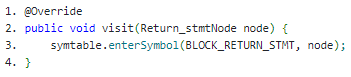
\includegraphics[scale=1.0]{figures/implementation/typeCecker/3-3-return-stmt-enter-symbol-table.png}}
\caption{If a return statement is encountered it, it is noted for the current scope.}
\label{lf05}
\end{figure}

\begin{figure}[H]
\centering
\frame{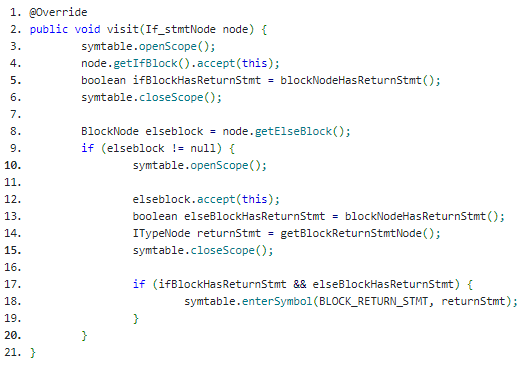
\includegraphics[scale=1.0]{figures/implementation/typeCecker/3-2-ifstmt-return-check.png}}
\caption{If an return statement in an if else block is guaranteed, it is noted for the current scope.} 
\label{lf05}
\end{figure}

 \begin{figure}[H]
\centering
\frame{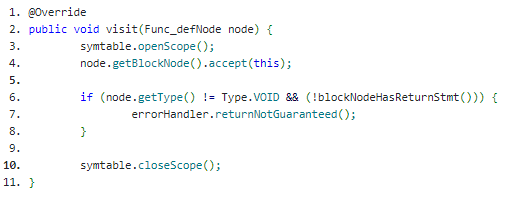
\includegraphics[scale=1.0]{figures/implementation/typeCecker/3-1-func-def-missing-return.png}}
\caption{If there is no return statement in the current scope, or an if else block where return is guaranteed throw an error.}
\label{lf05}
\end{figure}


